\documentclass[12pt]{article} % Документ принадлежит классу article, а также будет печататься в 12 пунктов.
\usepackage{array} % Для титульника
\usepackage{ucs}
\usepackage[utf8x]{inputenc} % Включаем поддержку UTF8
\usepackage[russian]{babel}  % Включаем пакет для поддержки русского языка
\usepackage[left=2cm,right=2cm, top=2cm,bottom=2cm,bindingoffset=0cm]{geometry} % Отступы по краям страницы
\usepackage{amssymb,amsfonts,amsmath,mathtext,cite,enumerate,float} % Математические штуки
\usepackage{cmap} % чтобы работал поиск по PDF
\usepackage{graphicx} % для вставки картинок

\usepackage{wrapfig} % Обтектание картинок текстом
 
%  для гиперссылок
\usepackage{xcolor}
\usepackage{hyperref}
\definecolor{linkcolor}{HTML}{191970} % цвет ссылок
\definecolor{urlcolor}{HTML}{191970} % цвет гиперссылок
\hypersetup{pdfstartview=FitH,  linkcolor=linkcolor,urlcolor=urlcolor, colorlinks=true}

\usepackage{pscyr} % Нормальные шрифты
\usepackage{setspace} % Для отступов между строк
%Это для формирования листингов
\usepackage{listings}
\lstset{inputencoding=cp1251, extendedchars=\true}
\lstdefinestyle{customc}{
	belowcaptionskip=2\baselineskip,
	breaklines=true,
	%frame=L,
	xleftmargin=\parindent,
	language=Matlab,
	showstringspaces=false,
	basicstyle=\ttfamily,
	keywordstyle=\bfseries\color{blue!40!black},
	commentstyle=\itshape\color{green!40!black},
	identifierstyle=\color{black},
	stringstyle=\color{purple},
}


\begin{document} % Начало документа

\title{Распознавание образов. Лабораторная работа №1. \\
	"Моделирование случайных величин".\\
	Вариант 6 (б): Распределение Рэлея}
\date{}
\author{\textit{Выполнил}: студент 4 курса, группы 6.1 \\
	Суходолов Денис}
        
\maketitle

\begin{spacing}{1} % Для отступов между строк
%\clearpage % Переход на новую страницу
\section{Код работы на MATLAB}
\lstinputlisting[caption=Распределение Рэлея, style=customc]{MyLab1Releigh.m}
\section{График зависимостей}
\begin{figure}[h]
	\begin{center}
		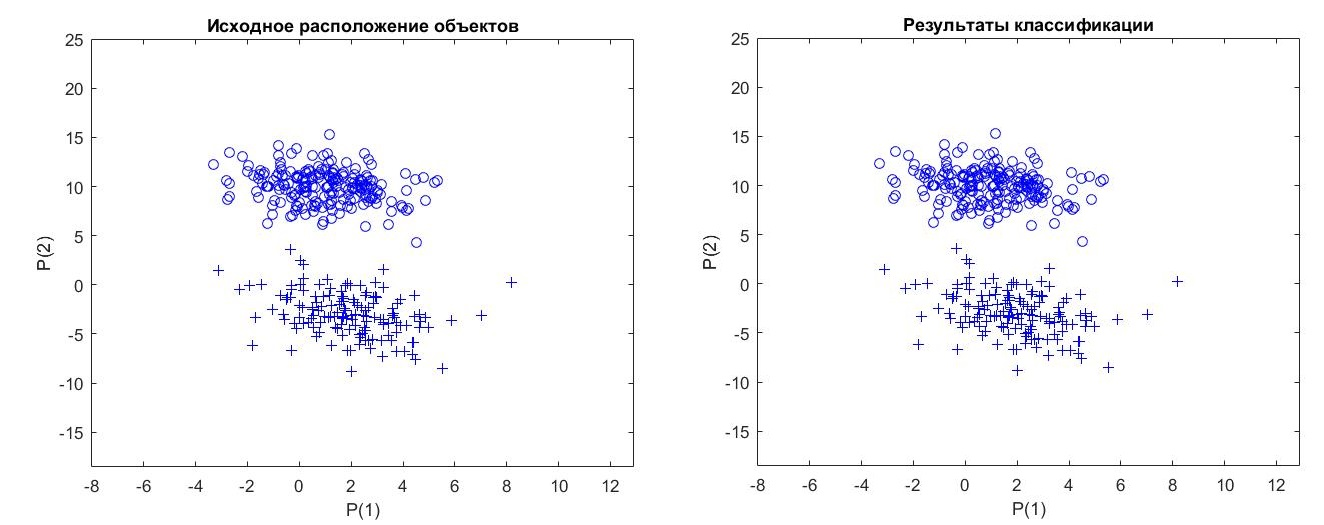
\includegraphics[width = 18cm]{1.jpg}
		\caption{Значение выборочной дисперсии}
	\end{center}
\end{figure}
~\\
































\end{spacing}
\end{document}